\documentclass[compress,red]{beamer}
\usetheme{Warsaw}
\useoutertheme[subsection=false]{smoothbars}

\usepackage{helvet}
\usepackage{graphicx}
\usepackage{booktabs}
\usepackage{hyperref}
\usepackage{url}

\usepackage{remreset}% tiny package containing just the \@removefromreset command
\makeatletter
\@removefromreset{subsection}{section}
\makeatother
\setcounter{subsection}{1}

\title[Managing equipment at CERN]%
	{A strategy for managing diverse equipment\\
	in the CERN controls group}
\author[Javier Serrano, David Cobas et al.]{%
	Javier Serrano, Juan David Gonz\'alez Cobas}
\date{FOSDEM'2012}

\begin{document}

% ------------------------------------------------------
\begin{frame}
\titlepage
\end{frame}

% ------------------------------------------------------
\begin{frame}{The FMC family of boards}

\begin{itemize}
\item carriers in PCIe and VME format
\item simple mezzanines with electronics for ADCs, DACs, DIO and endless
    other applications
\item circuitry in the mezzanine
\item FPGA application logic in the carrier
\item \emph{logic in the FPGA is organized as a set of IP cores
    interconnected through an internal bus named
    \textcolor{red}{Wishbone}}
\end{itemize}
\end{frame}

% ------------------------------------------------------
\begin{frame}
\begin{figure}[t]
   \centering
   \includegraphics[width=80mm]{adcarch.pdf}
   \caption{Block diagram of the FMC slow ADC application.}
   \label{slow-adc}
\end{figure}
\end{frame}

% ------------------------------------------------------
\begin{frame}
\begin{itemize}
\item Basic I${}^2$C interfacing to the mezzanine board.
\item Wishbone mastering.
\item DMA access to DDR3 memory in the carrier board.
\item Mezzanine-specific control logic (\emph{e.g.} ADC programming/setup).
\item Interrupt control.
\end{itemize}
\end{frame}

% ------------------------------------------------------
\begin{frame}{Drivers for the FMC family}
The main concepts for the design of these drivers are
\begin{itemize}
\pause
\item modular structure that reflects the core structure of the firmware
\pause
\item one-to-one mapping driver $\leftrightarrow$ core (usually)
\pause
\item ability to dynamically load bitstreams by application
\end{itemize}

\pause
On the whole, the driver for the carrier board acts as a basic firmware
loader and a bridge driver (with device enumeration
\emph{\`a la PCI)} between the host bus (PCIe, VME) and the FPGA
interconnection bus

\pause
It will be (we hope) the first Wishbone bus driver in the mainstream
kernel $\Rightarrow$ will to go upstream, timeliness
\end{frame}


% ------------------------------------------------------
\begin{frame}{Architecture of the FMC drivers}
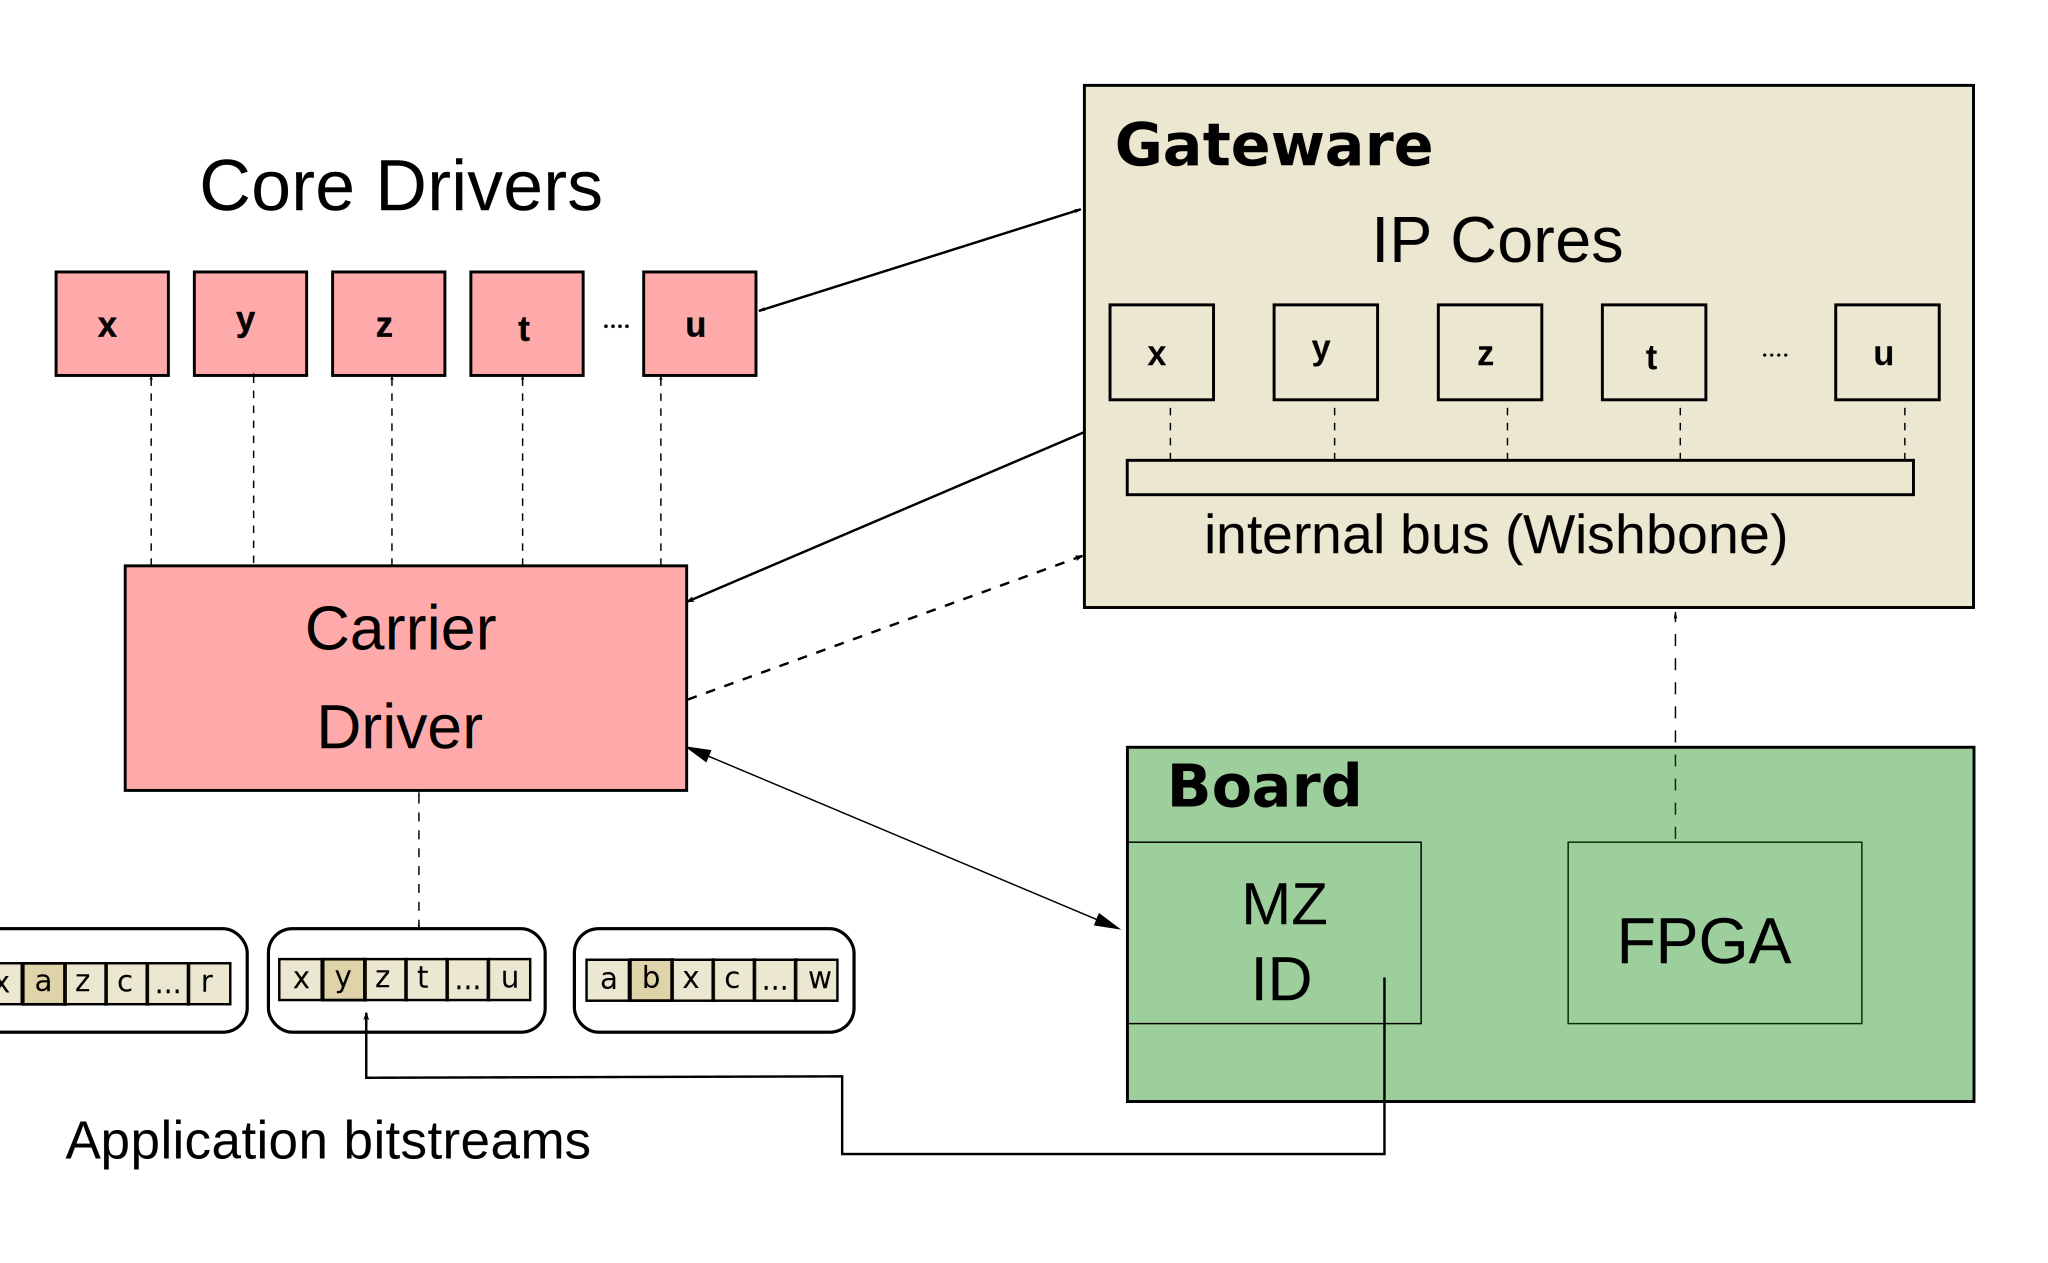
\includegraphics[height=0.8\textheight]{driverarch.pdf}
\end{frame}

% ------------------------------------------------------
\begin{frame}{How the FMC drivers start up}
\begin{itemize}
\item Identify the carrier board and initialize it.
\item Perform a basic identification of the mezzanine(s) installed in
    the FMC slot(s), and their configured applications.
\item Load the application firmware into the carrier FPGA.
\item Register a Wishbone bus with the kernel.
\item Enumerate the cores in that firmware (to wit, the
    inner blocks in figure~\ref{slow-adc}).
\item Register the devices those cores implement and install the drivers
    associated to them.
\end{itemize}
\end{frame}

\section{FMC boards}

% ------------------------------------------------------
\begin{frame}{A typical data acquisition application: carrier}
\begin{center}
\includegraphics[height=0.8\textheight]{spec.pdf}
\end{center}
\end{frame}

% ------------------------------------------------------
\begin{frame}{A typical data acquisition application: mezzanine}
\begin{center}
\includegraphics[rotate=180,height=0.7\textheight]{fmcadc.pdf}
\end{center}
\end{frame}


\section{The \texttt{zio} framework}

% ------------------------------------------------------
\begin{frame}{Industrial I/O frameworks}

\pause
\begin{block}{In Linux staging area}
\begin{itemize}
\item Comedi
\item IIO
\end{itemize}
\end{block}

\pause
\begin{block}{Drawbacks}
\begin{itemize}
\item do not suit our needs
\item interfaces are cumbersome
\end{itemize}
\end{block}

\pause
\begin{block}{Then \texttt{zio} comes}
\begin{itemize}
\item Alessandro Rubini and Federico Vaga, main developers
\item Integration mainstream \emph{ab initio}
\item See (soon) under \url{http://www.ohwr.org/}
\item \textcolor{red}{Clean design conforming to Linux kernel practice}
\end{itemize}
\end{block}

\end{frame}

% ------------------------------------------------------
\begin{frame}{Next candidates for (\texttt{zio}) integration}

CERN-developed drivers for
\begin{itemize}
\pause
\item Struck SIS33xx ADCs
\pause
\item Tews TPCI200/TVME200 carries plus IPOCTAL serial boards
\pause
\item all the CERN BE/CO-supported FMC boards in the Open Hardware Repository
\pause
\item timing receivers, White Rabbit, etc.
\end{itemize}
\end{frame}

\section{Conclusions and The Ultimate Goal}

% ------------------------------------------------------
\begin{frame}{Why did we do it?}

It gave us much more than we thought in the first place
\begin{itemize}
\pause
\item Smoother maintenance in the (frequent) case of\\
	kernel API changes.
\item Widespread distribution of the code base.
\item Contributing back to the the FOSS community.
\pause \color{red}
\item Very strict process of peer review of the code by knowledgeable
    and specialised maintainers.
\pause
\item Input (consulting!) from the topmost experts in the field.
\pause
\item Avoidance of suboptimal, \emph{ad hoc} solutions in favour of the
    best ones from the technical point of view.
\pause
\item Use of best practice and bleeding-edge tools selected by
    experienced programmers, \emph{e.g.} \texttt{git}, \texttt{sparse}
    and \texttt{coccinelle}.
\end{itemize}
\end{frame}

\end{document}
